\documentclass{article}
\usepackage{graphicx} % Required for inserting images
\usepackage{amsmath}
\usepackage[margin=1in]{geometry}
\usepackage{epigraph}
\usepackage{hyperref}

\title{Azienda 1 (gruppo 42)}
% \author{ Giacomo Biribicchi \and Marco Casu \and Ionut Cicio \and Christian Di Manno \and Alessandro Gautieri }
\date{}


\begin{document}

\maketitle

 \epigraph{The answer to the Ultimate Question of Life, the Universe, and Everything}{\textit{Douglas Adams \\ "The Hitchhiker's Guide to the Galaxy"}}

% Si vuole sviluppare un sistema informativo per la gestione dei dati sul personale di una certa azienda costituita da diversi dipartimenti. Durante la fase di raccolta dei requisiti è stata prodotta la specifica dei requisiti mostrata di seguito. Si chiede di iniziare la fase di Analisi dei requisiti ed in particolare di:

% raffinare la specifica dei requisiti eliminando inconsistenze, omissioni o ridondanze e produrre un elenco numerato di requisiti il meno ambiguo possibile
% produrre un diagramma UML delle classi concettuale che modelli i dati di interesse, utilizzando solo i costrutti di classe, associazione, attributo

\section{Requisiti}

I dati di interesse per il sistema sono \textbf{impiegati}, \textbf{dipartimenti}, \textbf{direttori} dei dipartimenti e \textbf{progetti} aziendali.

\paragraph{Impiegato}

% \textit{(se vogliamo essere pedanti, l'impiegato deve avere almeno 16 anni e al più 70, ma dipende dal ma dipende dal giorno in cui viene assunto, quindi è un requisito inutile)}

\begin{enumerate}
    \item Nome (include anche il doppio nome), cognome, data di nascita. 
    \item Stipendio attuale \textit{(dato che interessa solo lo stipendio attuale, non serve memorizzare lo storico degli stipendi)}.
    \item Dipartimento a cui afferisce, con relativa data di afferenza \textit{(esattamente uno)}.
    \item La data di afferenza al dipartimento non può essere precedente alla creazione dell'azienda.
    \item Uno stesso impiegato può dirigere più di un dipartimento.
    \item L'impiegato può partecipare a \textbf{0 o più progetti} \textit{(un nuovo impiegato non partecipa ancora a nessun progetto)}.
    \item Ogni dipendente può cambiare dipartimento, e vogliamo memorizzare lo storico dei dipartimenti in cui ha lavorato.
    \item L'associazione con la data più recente sarà considerata 
    quella valida/corrente.
    \item Un dirigente non afferisce al dipartimento che dirige. Afferisce al dipartimento riservato ai dirigenti.
\end{enumerate}

\paragraph{Dipartimento}

\begin{enumerate}
    \item Nome, telefono.
\end{enumerate}

\paragraph{Progetto}

\begin{enumerate}
    \item Ad un progetto possono partecipare \textbf{0 o più impiegati} \textit{(potrebbe succedere che il progetto è nuovo e non è stato assegnato nessun impiegato)}.
    \item Il budget di un progetto non può essere negativo. 
\end{enumerate}

% I dati di interesse per il sistema sono impiegati, dipartimenti, direttori dei dipartimenti e
% progetti aziendali.
% Di ogni impiegato interessa conoscere il nome, il cognome, la data di nascita e lo
% stipendio attuale, il dipartimento (esattamente uno) al quale afferisce.
% Di ogni dipartimento interessa conoscere il nome, il numero di telefono del centralino,
% e la data di afferenza di ognuno degli impiegati che vi lavorano.
% Di ogni dipartimento interessa conoscere inoltre il direttore, che è uno degli impiegati
% dell’azienda.
% Il sistema deve permettere di rappresentare i progetti aziendali nei quali sono coinvolti
% i diversi impiegati. Di ogni progetto interessa il nome ed il budget. Ogni impiegato può
% partecipare ad un numero qualsiasi di progetti.

% Di ogni impiegato interessa conoscere il nome, il cognome, la data di nascita, lo stipendio attuale e il dipartimento al quale afferisce (\textit{esattamente uno}, con la rispettiva data di afferenza).
% Di ogni dipartimento interessa conoscere il nome, il numero di telefono del centralino
% Di ogni dipartimento interessa conoscere inoltre il direttore, che è uno degli impiegati dell’azienda.
% Il sistema deve permettere di rappresentare i progetti aziendali nei quali sono coinvolti i diversi impiegati.
% Di ogni progetto interessa il nome ed il budget.
% Ogni impiegato può partecipare ad un numero qualsiasi di progetti.

\section{UML}

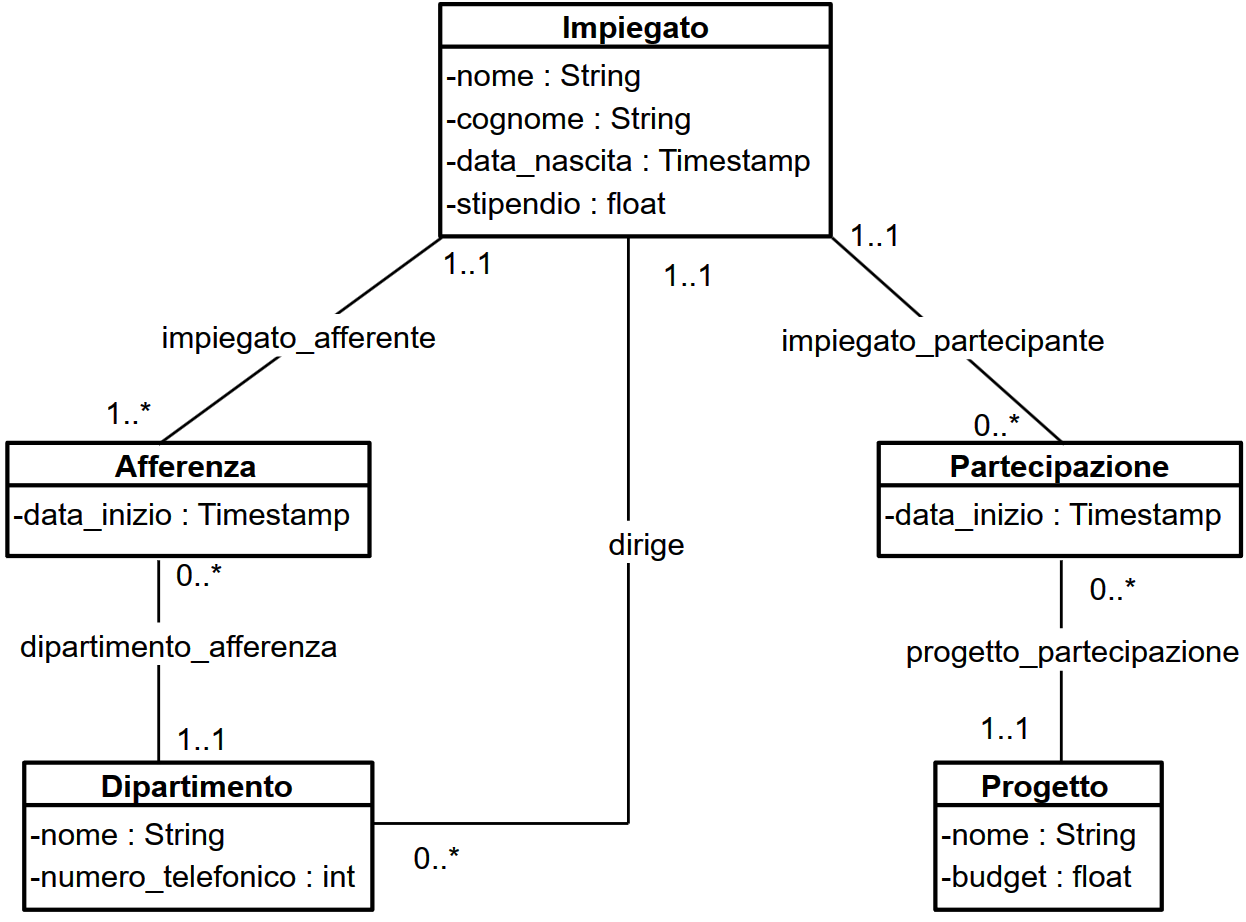
\includegraphics[width=\textwidth]{UML.png}


\end{document}
